%@+leo-ver=4-thin
%@+node:paran.20140605081907.1988:@shadow expirimentalResults.tex
%@@color
%@@language latex

\chapter{Experimental results}

\section{Purpose}
%@<<purpose>>
%@+node:paran.20140813185646.2164:<<purpose>>
The purpose of this experiment is to measure how many insertions, deletion and modifications are performed on the Java AST verses comments across a range of realistic benchmarks. Similarly, how many insert and delete pairs can be classified as moves.

%@+at
% establish if there are superficial changes in currently working projects.  
% By superficial we mean that the change does not add much of value apart from 
% personal taste or formatting.  In some cases changes to the order of methods 
% within a class does change the behaviour of a program, this is an example of 
% a superficial change.  It is harder to determine if comments are superficial 
% because certain comments could be important to others and others irrelevant. 
% We will attempt to establish if there are any patterns in comments to 
% determine if they are superficial or not.  Determining if there are 
% superficial change may indicate that there is a separation between personal 
% preferences that would be best contained in a private view and items that 
% need to be shared for collaboration.
%@-at
%@@c
%@nonl
%@-node:paran.20140813185646.2164:<<purpose>>
%@nl

\section{Methodology}
%@<<Methodology>>
%@+node:paran.20140813185646.2165:<<Methodology>>
We will now outline the experimental methodology. Our goal is make it possible for someone to reproduce our experiment.

%@<<setup>>
%@+node:paran.20140813185646.2166:<<setup>>
The experiment was run on a Lenovo laptop with 3.5GB Ram and 113.2 GB disk space assigned to the 64 bit Ubuntu 13.10 (Saucy Salamander) operating system. The tests were written in Java and run within the Eclipse IDE


%@-node:paran.20140813185646.2166:<<setup>>
%@nl

%@<<baselines>>
%@+node:paran.20140814214911.2179:<<baselines>>
 
 
 \begin{table}[p!]
    \small{
    \begin{tabular}{l|lllll}
    Benchmark        & Description   & Commits  & LOC   \\ \hline
    Jasm             &  \begin{minipage}[t]{0.5\textwidth}
Java bytecode assembler written for use with the Whiley programming language.

github.com/Whiley/Jasm 
\end{minipage}        & 74      & 29139 \\ \hline
    Jpp              & \begin{minipage}[t]{0.5\textwidth}
    Pre-processor for Java based on Bash shell script.
    
github.com/maandree/jpp
\end{minipage}        & 40      & 254   \\ \hline
    AST Java         & \begin{minipage}[t]{0.5\textwidth}
    Small parser written to transform Java into an AST.
    
github.com/klangner/ast-java 
\end{minipage}       & 24      & 10174 \\ \hline
\begin{minipage}[t]{0.15\textwidth}Java Object Diff\end{minipage} & \begin{minipage}[t]{0.5\textwidth}
Allows two Java objects to be compared at runtime.
     
github.com/SQiShER/java-object-diff 
\end{minipage}        & 291     & 10023 \\ \hline
    DiffJ            & \begin{minipage}[t]{0.5\textwidth}
    Diff tool which in addition to ignoring white space ignores changes of ordering in package names for a Java file.
    
github.com/jpace/diffj
\end{minipage}        & 490     & 13712 \\ \hline
    IRE              & \begin{minipage}[t]{0.5\textwidth}
    Java library for regular expression matching.
    
github.com/jkff/ire  
\end{minipage}       & 41      & 2714  \\ \hline
    Syntax           & \begin{minipage}[t]{0.5\textwidth}
    Compiler compiler used for teaching. 
    
github.com/jaimegarza/syntax 
\end{minipage}        & 89      & 9376  \\ \hline

    Auto Refactor           & \begin{minipage}[t]{0.5\textwidth}
    Eclipse plug-in that automatically refactors code 
    
github.com/JnRouvignac/AutoRefactor 
\end{minipage}        & 212      & 13400  \\ \hline
    \end{tabular}
    }
    \caption{A range of benchmarks that will be included in the test}
    \label{tab:benchmarks}
\end{table}
 
%@+at
% 
% The Refactor Categories Tool analyses all the historical changes ever made 
% on a software project by extracting successive revisions from a Git 
% repository using JGit.  Once we have two revisions we need to compare them.  
% To do this we compare each of the Java files in both revisions one by one. 
% We only test the Java file if it has been modified or renamed.  If the file 
% been inserted or deleted we ignore it because there is no way to make a 
% comparison. Once we have established that Java files exist, both in the 
% original and the updated copy, we use the text diff in JGit to compare them. 
% As outlined in section \ref{matchingTextWithAST} we figure out which AST 
% nodes the text changes contain.
% The Refactor Categories Tool splits up the identified blocks of source code 
% into several AST nodes and identifies anything between AST Nodes as being 
% text. @c
%@-at
%@nonl
%@-node:paran.20140814214911.2179:<<baselines>>
%@nl
%@<<how conducted>>
%@+node:paran.20140814214911.2180:<<how conducted>>
This text is further evaluated to determine if it is a change to comments or a change to white space. 
An example of this is if the text comparison detects a single change that inserts two new methods and a comment.  
The Refactor Categories Tool will recognise this as three distinct changes. 
This means that it is possible for the Refactor Categories Tool to notice more changes than a text based comparison. 

We had some garbage collection memory issues with some benchmarks that we were testing. 
To resolve these issues the Refactor Categories Tool was run individually once for each benchmark to further ensure that there were no memory leaks between runs.
We also increased the memory by changing the parameters for the run configuration.  The following parameters were added to the run configuration for the test.

\begin{verbatim}
-Xms512M 
-Xmx4096M
\end{verbatim}



%@+at
% There are a number of comparison operations that the refactor categories 
% tool investigates
% 
% \begin{description}
% 
%   \item [Delete]
%   <<del>>
%   \item [Insert]
%   <<ins>>
% 
%   \item [Modify]
%   <<mod>>
%   \item [Move]
%   <<mov>>
%   \item [Rename]
%   <<ren>>
%   \item [Equivalent]
%   <<eqv>>
% \end{description}
%  @c
%@-at
%@+at
% renames are determined as being something where although the AST label has 
% changed the type of the AST node remains the same and its contents have not 
% been changed in any way.
%@-at
%@@c  

%@-node:paran.20140814214911.2180:<<how conducted>>
%@nl
%@nonl
%@-node:paran.20140813185646.2165:<<Methodology>>
%@nl


\section{Results}
%@<<Results>>
%@+node:paran.20140814214911.2176:<<Results>>
\subsection{Overview}
%@<<overview>>
%@+node:paran.20140814214911.2177:<<overview>>
After running the Refactor Categories Tool over our benchmark suite we obtained the results shown in Table \ref{tab:results}

\begin{table}[!p]
    \small
    \begin{tabular}{l|llllll|l|lll}
    Benchmark        & \multicolumn{6}{|c|}{Java}           & WS & \multicolumn{3}{|c}{Comments} \\ \cline{2-7} \cline{9-11}
    ~                & Ins  & Del  & Mod  & Mov & Ren & Eqv & ~          & Ins      & Del & Mod  \\ \hline
    Jasm             & 264  & 76   & 385  & 7   & 0   & 0   & 26         & 7        & 6   & 95   \\
    Jpp              & 43   & 9    & 50   & 0   & 0   & 0   & 6          & 1        & 2   & 11   \\
    AST Java         & 87   & 28   & 72   & 1   & 0   & 11  & 5          & 2        & 0   & 22   \\
    \begin{minipage}[t]{0.15\textwidth}Java Object Diff\end{minipage} & 2645 & 1961 & 8862 & 5   & 9   & 187 & 270        & 52       & 25 & 881 \\
    DiffJ            & 3106 & 3164 & 5192 & 58  & 82  & 18  & 276        & 36       & 39  & 291  \\
    IRE              & 263  & 213  & 640  & 1   & 2   & 30  & 49         & 10       & 3   & 79   \\
    Syntax           & 1142 & 544  & 2216 & 6   & 7   & 12  & 204        & 14       & 81  & 451  \\
    Auto refactor    & 1702 & 1621 & 2809 & 7   & 16  & 25  & 295        & 30       & 16  & 568  \\
    \end{tabular}
    \caption{Results over our benchmark suite showing the number of inserts (Ins), deletes (Del), modifications (Mod), moves (Mov), renames (Ren) and equivalences (Eqv) for Java AST nodes, comments and white-space (WS) changes}
    \label{tab:results}
\end{table}

The number of text changes that were recognised during ordinary text comparison done using JGit for each benchmark are shown in Table \ref{tab:textcomp}. This table allows us to show the difference between an ordinary text merge (reported by JGit) and the results produced by the Refactor Categories Tool shown in Table \ref{tab:results}. Note that the values in this table are lower as the Refactor Categories tool detects multiple changes which a text based comparison aggregates.  

\begin{table}[!p]
    \centering
    \begin{tabular}{l|lll}
    Benchmark        & \multicolumn{3}{|c}{Ordinary Text Diff (reported by JGit)} \\ \hline
    ~                & Ins            & Del & Mod  \\ \hline
    Jasm             & 91             & 44  & 337  \\
    Jpp              & 23             & 3   & 41   \\
    AST Java         & 44             & 15  & 85   \\
    Java Object Diff & 1186           & 837 & 8219 \\
    DiffJ            & 746            & 991 & 3544 \\
    IRE              & 112            & 49  & 465  \\
    Syntax           & 691            & 214 & 1863 \\
    Auto Refactor    & 639            & 309 & 1621 \\
    \end{tabular}
    \caption{The result of doing an ordinary text comparison showing the number of inserts (Ins), deletes (Del) and modifications (Mod)}
    \label{tab:textcomp}
\end{table}



  
%@nonl
%@-node:paran.20140814214911.2177:<<overview>>
%@nl
\subsection{Discussion}
%@<<examination>>
%@+node:paran.20140814214911.2178:<<examination>>
%@<<figures>>
%@+node:paran.20140827082213.3569:<<figures>>
Figure \ref{fig:textDifference}, which has been generated from the data in Table \ref{tab:textcomp}, shows the average for all the benchmarks of the types of operations found during an ordinary text comparison.  
Figure \ref{fig:javaDifference}, which has been generated from the data in Table \ref{tab:results}, shows the average for all the benchmarks of the types of operations found during a Java AST node comparison.

%\begin{minipage}[t]{1\textwidth}
\begin{figure}[p] 
 \begin{center}
 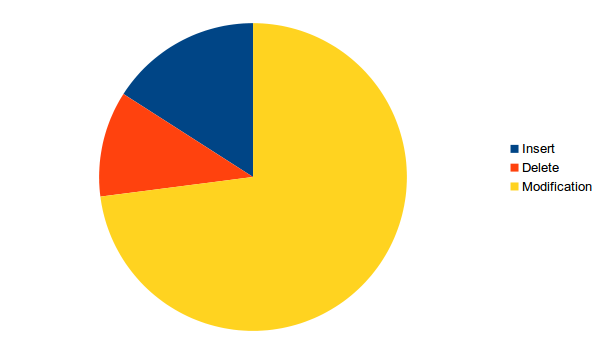
\includegraphics[scale=.8]{TextDifference}
 \end{center}
 \caption{Type of operations for an ordinary text comparison on average for all the benchmarks}
 \label{fig:textDifference}
\end{figure}

\begin{figure}[p] 
 \begin{center}
 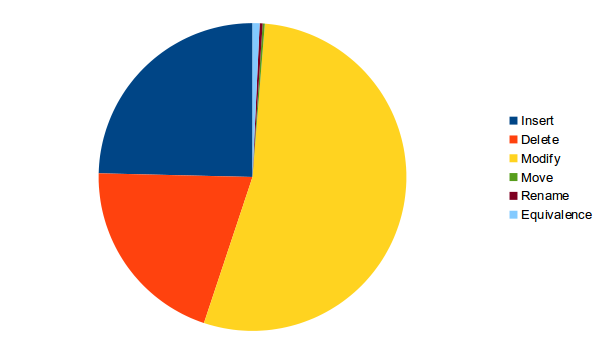
\includegraphics[scale=.8]{JavaDiff}
 \end{center}
 \caption{Type of operations for a Java AST node comparison on average for all the benchmarks}
 \label{fig:javaDifference}
\end{figure}
%\end{minipage}
%@nonl
%@-node:paran.20140827082213.3569:<<figures>>
%@nl

When we compare the figures the number of modifications is different.
The percentage is much higher in the text comparison that JGit normally uses and lower for the Refactor Categories tool.
The reason for this is because a change done to a block of text recorded in the \lstinline{EditList} object is made up of a number of smaller changes.  
For instance a single line detected by the JGit text comparison may contain a Java AST node change and a change to a comment.
The Refactor Categories Tool records each of these changes separately.
A change detected by JGit could be a number of lines, so a single block of text could contain multiple Java AST nodes.  
If a block of text is a delete all the Java AST nodes or comments in that range will also be deletes. 
If a block of text is an insert all the Java AST node or comments in that range will also be inserts.
It is slightly different for blocks of text that have been modified.
It is possible that some of the changes could be Java AST nodes or comments that have been inserted.
They could also be deletes rather than modifications.
Some of the changes that an ordinary text diff recognises as modifications could actually be made up of individual inserts and deletes.
Note that the number of changes reported by the Refactor Categories Tool will increase exactly for this reason.
Furthermore, when we examine these changes more closely using the Refactor Categories Tool the comparative percentage of insert and delete increases while the percentage of modifications tends to decrease.  

Instead of having insert, delete and modifications Figure \ref{fig:javaDifference} also has move and rename.
Predominately the changes were still identified as modifications, inserts and deletes rather than the move and rename we are interested in.
What this could mean is although some non-functional changes have been introduced it does not occur very often.  
However, it is also possible that a more advanced identification algorithm could improve the results. 

%@<<comments>>
%@+node:paran.20140827082213.3570:<<comments>>
Another aspect we were interested in was the difference between Java based differences and non-Java changes such as comments or white-space.
Figure \ref{fig:changeType} shows the how many Java changes were detected as compared to comments and white-space.
This shows that the predominate change in the source code was a change in functionality rather than a change to the documentation.
It implies that in programming projects there tends to be many more lines of program than lines of comments.
What this means for this thesis is that currently there are more changes to functionality rather than to coding style and documentation.
As there are still significant amount of changes to comments it is possible that being able to modify comments that will not be merged could be useful.  

Figure \ref{fig:commentsPie} more closely examines the type of changes that have occurred to comments in the source code.
By far the main change to comments is modification.
Unlike Java AST Nodes blocks of code containing comments are not further divided.
This means that the block of code marked as a modification to a comment may in fact contain a number of deletes or inserts.
Another possible cause for a large number of comment changes to be modification is if a programming project is well established.
It is possible, in an existing project, that changes are made to the code and the existing comments are modified to reflect that change.
The changes to the code could include insert or deletes in addition to modifications to the source code.
In this situation when comparing the amount of inserts, deletes and modifications between the source code changes and the comment changes the source code will have comparatively more inserts and deletes whilst the comments will have comparatively more modifications.

%\begin{minipage}[t]{1\textwidth}
\begin{figure}[p] 
 \begin{center}
 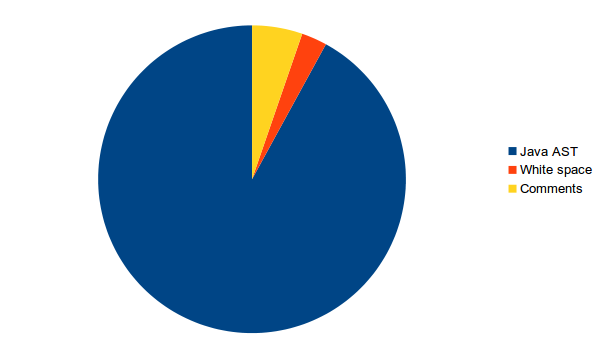
\includegraphics[scale=.8]{changeTypePie}
 \end{center}
 \caption{The type of changes that most often occurred over all the benchmarks}
 \label{fig:changeType}
\end{figure}

\begin{figure}[p] 
 \begin{center}
 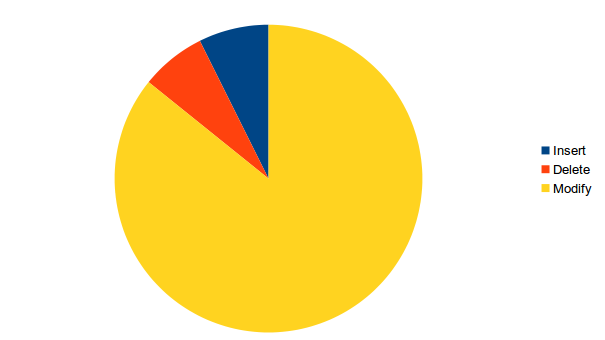
\includegraphics[scale=.8]{Comments}
 \end{center}
 \caption{Types of operations for comments on average over the benchmarks}
 \label{fig:commentsPie}
\end{figure} ~\\
%\end{minipage}

A significant number of comments have been inserted and deleted.
Examining these items a little closer revealed that some included the words "TODO" or "FIXME".
Although the addition of these comments are likely to be associated with a related code change they may only be relevant to people working on that section of the code.
The same is true for blocks of commented out code.
In this situation having a private view could be useful.
%@nonl
%@-node:paran.20140827082213.3570:<<comments>>
%@nl



%@+at
% Although the Refactor Categories tool tested to see if comments moved none 
% were detected across the benchmarks.
%@-at
%@@c


%@+at
% There were a number of benchmarks we would have liked to have used but due 
% to memory constraints we had to omit these from the benchmark suite.
% 
% 
% 
%  \begin{table}[H]
%     \small{
%     \begin{tabular}{l|lllll}
%     Benchmark        & Description   & Commits  & LOC   \\ \hline
%     Antlr4             &  \begin{minipage}[t]{0.5\textwidth}
%     A parser generator used to create programming grammers.
% 
% github.com/antlr/antlr4
% \end{minipage}        & 2867      & 40373 \\
% 
%     Clojure             & \begin{minipage}[t]{0.5\textwidth}
%     A programming language that targets the JVM
% github.com/clojure/clojure
% \end{minipage}        & 2602      & 37512   \\
%     gitblit         & \begin{minipage}[t]{0.5\textwidth}
%      Java implementation of Git.
% github.com/gitblit/gitblit
% \end{minipage}       & 2334       & 72188 \\
%     Jacoco            & \begin{minipage}[t]{0.5\textwidth}
%     Library used to determine code coverage.
% github.com/jacoco/jacoco
% \end{minipage}        & 1184     & 25357 \\
%     JGit             & \begin{minipage}[t]{0.5\textwidth}
%     Java implementation of Git developed by the Eclipse Foundation.
% eclipse.org/jgit
% \end{minipage}       & 3285      & 137993  \\
%     Lombok           & \begin{minipage}[t]{0.5\textwidth}
%     A library that used annotaions to extend Java.
% github.com/rzwitserloot/lombok
% \end{minipage}        & 1624      & 39154  \\
%     Revori           & \begin{minipage}[t]{0.5\textwidth}
%     A revision based DBMS.
% github.com/ReadyTalk/revori
% \end{minipage}        & 349      & 18931  \\
%     \end{tabular}
%     }
% \end{table}
% 
%@-at
%@@c

%@+at
% 
% 
% Memory issues
% baselines we could not compare
% the greater the amount of revisions the more chance that there was a memory 
% error
% 
%@-at
%@@c
%@nonl
%@-node:paran.20140814214911.2178:<<examination>>
%@nl
%@nonl
%@-node:paran.20140814214911.2176:<<Results>>
%@nl

%@+at
% The data sets following are complete git repositories which have been 
% examined to discover the proportion of changes to behaviour compared to 
% ascetic changes that do not affect the behaviour of the program.
% 
% 
% in table ~\ref{tab:DataSets}
% 
% \begin{table}
%   \caption{Complete git repositories that are tested}
%   \label{tab:DataSets}
%   \begin{center}
%     \begin{tabular}{|c|c|c|}
%        Jasm & this a a Java bytecode assembler
%        written for use with the Whiley programming language. & 
% https://github.com/Whiley/Jasm\\
%       foo & bar \\
%     \end{tabular}
%   \end{center}
% \end{table}
% 
%@-at
%@@c

%@+at
% 
% 
% 
% There are a number of Java categories that the Refactor Categories Tool will 
% recognise.  Apart from the traditional insert, delete and modify it will 
% also recognise if an AST Node has been renamed but the content and type of 
% the node remains the same.  It will recognise valid moves within a scope. It 
% will also recognise when the text based merge got it wrong by claiming that 
% the code was not functionally equivalent when in fact it was.
% 
% Apart from this it will also differentiate between Java code and comments.  
% It can tell if comments have been inserted, modified, moved or deleted.  It 
% will also pick up any changes to that white-space that have not already been 
% figured out by the text based comparison.
%@-at
%@@c
 
%@+at
% Comments
%     Insert
%     Delete
%     Modify
%     Move
% White space
%    Modify
% 
% Java
%  Insert
%  Delete
%  Modify
%  Move
%  Rename
%@-at
%@@c


%@+at
% need the results in here
% 
% 
% what this means
% modifications to comments
% 
% modification to comments could be surplus to need
% 
% 
% Examine certain events
% 
% in this case the comment is removed but as the comment is associated with a 
% functional change the comment also needs to change in both versions
%@-at
%@@c
%@@c
%@-node:paran.20140605081907.1988:@shadow expirimentalResults.tex
%@-leo
